\documentclass{article}
\usepackage{tikz}
\usetikzlibrary{decorations.markings}

\begin{document}

\begin{figure}[h]
    \centering
    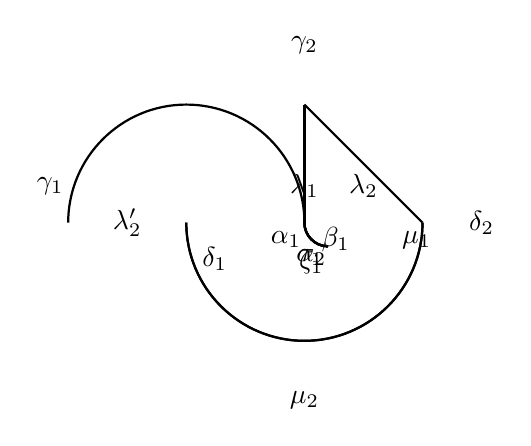
\begin{tikzpicture}[scale=1.5]
        % Define coordinates for the points
        \coordinate (A) at (-1,0);
        \coordinate (B) at (0,0);
        \coordinate (C) at (1,0);
        \coordinate (D) at (0,1);
        
        % Draw the arcs and lines
        \draw[thick] (A) arc (180:360:1) node[pos=0.9, above] {$\mu_1$};
        \draw[thick] (B) arc (0:180:1) node[pos=0.9, left] {$\gamma_1$};
        \draw[thick] (C) arc (0:-180:1) node[pos=0.9, right] {$\delta_1$};
        \draw[thick] (D) -- (B) node[pos=0.5, below] {$\lambda_1$};
        \draw[thick] (D) -- (C) node[pos=0.5, below] {$\lambda_2$};
        
        % Draw the small arcs and labels
        \draw[thick] (B) arc (180:270:0.2) node[pos=0.5, left] {$\alpha_1$};
        \draw[thick] (B) arc (180:270:0.2) node[pos=0.5, right] {$\beta_1$};
        \draw[thick] (B) arc (180:270:0.2) node[pos=0.5, below] {$\tau_1$};
        \draw[thick] (B) arc (180:270:0.2) node[pos=0.5, below] {$\zeta_1$};
        \draw[thick] (B) arc (180:270:0.2) node[pos=0.5, below] {$\alpha_2$};
        
        % Draw the labels for the complementary arcs
        \node at (0,-1.5) {$\mu_2$};
        \node at (0,1.5) {$\gamma_2$};
        \node at (1.5,0) {$\delta_2$};
        \node at (-1.5,0) {$\lambda_2'$};
    \end{tikzpicture}
    \caption{Left: Partial and whole spherical linkage of a mesh in Fig.~\ref{sqmesh}, $(\lambda_i, \gamma_i, \mu_i, \delta_i, \alpha_i, \beta_i)$ and $(\lambda_i', \gamma_i', \mu_i', \delta_i', \alpha_i', \beta_i')$ are complementary to $\pi$ respectively, the gap between $\beta_1$ and $\alpha_2$ is caused by $\tau_1$ and $\zeta_1$.}
    \label{fig:spherical_linkage}
\end{figure}

\end{document}